
\documentclass{article}


\usepackage{amsfonts}
\usepackage{amsmath}
\usepackage{fancyhdr}
\usepackage{framed}
\usepackage[margin=1in]{geometry}

\pagestyle{fancy}
\fancyfoot[RE,RO]{
  \sc \footnotesize
  SMGT 435: Baseball Analytics\\
  \copyright~2024 Scott Powers}


\usepackage{tikz}
\usetikzlibrary{decorations.pathmorphing}

\begin{document}

\begin{framed}
  {\bf Caution:} These lecture notes are under construction. You may find parts that are incomplete.
\end{framed}

\setcounter{section}{4}
\section{\sc Pitch Outcome Modeling}

  At first glance, there are a lot of tracking metrics reported on each pitch: extension, release x/y, speed, plate location x/y, horizontal break, vertical break, induced vertical break, time to plate, etc. But which of these pieces of information are redundant, and are we missing any information? Here it helps to understand how the pitch moves and how we get these measurements.

  \subsection{\sc Basic Physics of Ball Flight}

    There are a few known forces acting on a pitch baseball during its flight from the pitcher's hand toward home plate. The simplest force is {\bf gravity}, which pulls the ball down toward the ground at a constant acceleration of approximately 32.17 feet per second per second. The direction of the gravity force is constant, always pointing directly down toward the ground.

    The other forces come from fluid dynamics and have to do with the movement of air around the baseball. These are {\bf drag} force (aka air resistance), {\bf lift} force (aka Magnus force) and {\bf side} force (aka seam-shifted wake). The magnitudes of these three forces are given by
    \begin{align*}
      F_D &= C_D \rho A v^2 / 2\\
      F_L &= C_L \rho A v^2 / 2\\
      F_S &= C_S \rho A v^2 / 2,
    \end{align*}
    where $\rho$ is the air density; $A$ is the cross-sectional area of the ball; and $v$ is the speed of the ball, i.e. the magnitude of its velocity vector. The drag coefficient $C_D$ depends on properties of the baseball and is subject to variation through the manufacturing process (although this matters more for batted balls than for pitched balls). The lift coefficient $C_L$ is proportional to the angular velocity (i.e. spin rate) of the baseball.\footnote{Nathan A (2007) ``The effect of spin on the flight of a baseball'' {\it American Journal of Physics} {\bf 74}, 658--664.} The side-force coefficient $C_S$ depends on the difference in roughness (primarily due to seam orientation) of the ball between the two poles of the axis of rotation.\footnote{Cross R (2012) ``Aerodynamics in the classroom and at the ball park'' {\it American Journal of Physics} {\bf 80}, 289--297.}
    
    Drag pushes against the baseball in the direction opposite its velocity vector. The pitcher has very little control over this beyond the speed of the pitch. Lift is the primary way pitchers impart movement on the baseball, by spinning it. This force is the reason that fastballs, curveballs and sliders all move differently from each other. It pushes the ball in a direction matching the cross product of the velocity vector and the angular velocity vector. Side force received a lot of attention in the early 2020s. If one side of the baseball is consistently rougher than the other while the baseball spins, this force will push the baseball in the direction of the smoother side. Note that drag, lift and side force are not constant throughout the flight of a pitch.
 
  \subsection{\sc Data Generation}

    Historically, the way that data vendors have provided pitch tracking data to MLB teams is by taking snapshots of the location of the pitch during its flight and then fitting a three-dimensional quadratic curve to the location of the baseball as a function of time. All of the pitch tracking metrics depend only on this quadratic curve, not on the raw measurements. For example, the technology might capture the location of the baseball at 25 Hz (i.e. 25 frames per second). Because typical pitch takes about 10 seconds from release to reach home plate, this means we would have 10 observed locations of the pitch along its trajectory. By fitting a quadratic polynomial to the trajectory, data vendors are effectively assuming that the acceleration vector is constant for the flight of the pitch. All tracking metrics are based on this assumption.

    We describe the pitch as moving through $(x, y, z)$ space, where the $x$ direction is from the pitching rubber to first base ($x = 0$ is the center of home plate); the $y$ direction is from the pitching rubber to second base ($y = 0$ is the back of home plate); and the $z$ direction is from the pitching rubber to the sky ($z = 0$ is the ground). Using a quadratic approximation to the flight of the pitch, the position of the ball at time $t$ can be written as $(x(t), y(t), z(t))$, where
    \begin{align*}
      x(t) &= a_x t^2 / 2 + b_x t + c_x\\
      y(t) &= a_y t^2 / 2 + b_y t + c_y\\
      z(t) &= a_z t^2 / 2 + b_z t + c_z.
    \end{align*}
    This collection of quadratic coefficients $a_x, b_x, c_x, a_y, b_y, c_y, a_z, b_z, c_z$ is sufficent for describing all of the data provided by the vendor (aside from spin rate and spin axis, if applicable). In other words, if you have these quadratic coefficients, you can calculate all of the pitch tracking metrics.
  
  \subsection{\sc TrackMan Metrics}

    TrackMan is a Danish company that was the provider of pitch and batted ball tracking data for MLB from 2017 through 2019. Their Doppler radar system beat out San Francisco-based Sportvision's computer vision system for the league contract because it could pick up the pitch at release. Sportvision's PITCHf/x product started tracking the ball when it was 50 feet away from the back of home plate.

    Despite TrackMan's short run as the league's vendor for ball tracking data, the company had a big impact on the metrics used to describe pitch flight. When London-based Hawk-Eye took over the league contract with a new computer vision system starting in 2020, they used their own technology to produce metrics matching TrackMan's definitions because teams were already familiar with these.

    The first handful of metrics are straightforward to calculate from the quadratic coefficients. The only noteworthy step is using the quadratic equation to calculate the time at which the pitch cross the front of home plate ($y = 17/12$).
    \begin{align*}
      \mbox{Release Point X} &= c_x\\
      \mbox{Release Point Z} &= c_z\\
      \mbox{Extension} &= 60.5 - c_y\\
      \mbox{Release Speed} &= \sqrt{b_x^2 + b_y^2 + b_z^2}\\
      \mbox{Plate Time} \equiv t_p &= \left(-b_y - \sqrt{b_y^2 - 4 * (a_y / 2) * (c_y - 17 / 12)}\right) / a_y\\
      \mbox{Plate Location X} &= a_x t_p^2 / 2 + b_x t_p + c_x\\
      \mbox{Plate Location Z} &= a_z t_p^2 / 2 + b_z t_p + c_z
    \end{align*}

    Calculating horizontal and vertical breaks is slightly more complicated. For horizontal and vertical break, we calculate where the pitch would cross the plate if it travelled a straight line following the initial velocity vector at release. For induced vertical break, we calculate where the pitch would cross the plate if gravity were the only force acting on it from release. Break is defined as the difference between the observed plate location and these hypothetical break locations.
    \begin{align*}
      \mbox{Plate Location X (Line)} &= b_x t_p + c_x\\
      \mbox{Horizontal Break} &= \mbox{Plate Location X} - \mbox{Plate Location X (Line)}
    \end{align*}
    \begin{align*}
      \mbox{Plate Location Z (Line)} &= b_z t_p + c_z\\
      \mbox{Vertical Break} &= \mbox{Plate Location Z} - \mbox{Plate Location Z (Line)}
    \end{align*}
    \begin{align*}
      \mbox{Plate Location Z (Gravity)} &= -32.17 \cdot t_p^2 / 2 + b_z t_p + c_z\\
      \mbox{Induced Vertical Break} &= \mbox{Plate Location Z} - \mbox{Plate Location Z (Gravity)}
    \end{align*}
    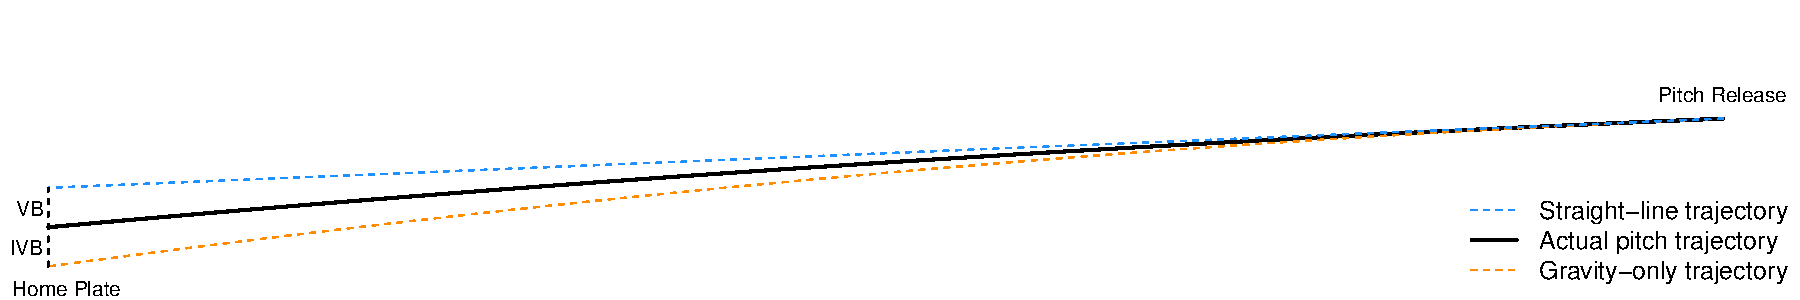
\includegraphics[width = \textwidth]{figures/vertical_break_illustration.pdf}

  
  \subsection{\sc Pitch Outcome Model}

    To summarize what we have learned in this chapter, the vector $\vec v = (a_x, b_x, c_x, a_y, b_y, c_y, a_z, b_z, c_z$) of quadratic coefficients is sufficient for describing the estimated path of the pitch (which is all we get from the data provider). In other words, if these quadratic coefficients are known, any other metric is known (and possible to calculate). In this sense, we can think of the quadratic coefficients as a canonical representation of pitch tracking data.
    
    We revisit the pitch outcome tree from the previous chapter.

    \begin{center}
      \begin{tikzpicture}
        \node (pitch) at (0, 0) {\small Pitch};
        \node (take) at (-3, -1.2) {\small Take};
        \node (swing) at (3, -1.2) {\small Swing};
        \node (call) at (-4.5, -2.4) {\small Call};
        \node (hbp) at (-1.5, -2.4) {\small HBP};
        \node (miss) at (1.5, -2.4) {\small Miss};
        \node (contact) at (4.5, -2.4) {\small Contact};
        \node (ball) at (-6, -3.6) {\small Ball};
        \node (strike) at (-3, -3.6) {\small Strike};
        \node (foul) at (3, -3.6) {\small Foul};
        \node (fair) at (6, -3.6) {\small Fair};
        \node (outcome) at (6, -4.8) {\small Outcome};
        \draw[->] (pitch) -- (take);
        \draw[->] (pitch) -- (swing);
        \draw[->] (take) -- (call);
        \draw[->] (take) -- (hbp);
        \draw[->] (swing) -- (miss);
        \draw[->] (swing) -- (contact);
        \draw[->] (call) -- (ball);
        \draw[->] (call) -- (strike);
        \draw[->] (contact) -- (foul);
        \draw[->] (contact) -- (fair);
        \draw[->, decorate, decoration = snake] (fair) -- (outcome);
      \end{tikzpicture}
    \end{center}

    One common approach to pitch outcome modeling is to estimate the probability of each binary split in the outcome tree, conditional on the pitch tracking data $\vec v$ and a vector $\vec c$ of contextual features (e.g. count). A sixth regression function models the expected linear weight of the outcome, conditional on the ball being put into to play. The six models to estimate are:
    \begin{align*}
      f_1(\vec v, \vec c) &= \mathbb{P}(\mbox{Swing} \mid \vec v, \vec c)\\
      f_2(\vec v, \vec c) &= \mathbb{P}(\mbox{HBP} \mid \vec v, \vec c, \mbox{Take})\\
      f_3(\vec v, \vec c) &= \mathbb{P}(\mbox{Strike} \mid \vec v, \vec c, \mbox{Call})\\
      f_4(\vec v, \vec c) &= \mathbb{P}(\mbox{Contact} \mid \vec v, \vec c, \mbox{Swing})\\
      f_5(\vec v, \vec c) &= \mathbb{P}(\mbox{Fair} \mid \vec v, \vec c, \mbox{Contact})\\
      f_6(\vec v, \vec c) &= \mathbb{E}[\mbox{Outcome} \mid \vec v, \vec c, \mbox{Fair}].
    \end{align*}

    Estimating each of these regression models is a supervised learning task.\footnote{To learn more about supervised learning, see STAT 413.} Approaches generally fall into two categories. The first approach is to use more traditional regression techniques (logistic regression, linear regression) with careful feature engineering. In this case, it is important to construct features that have clear, interpretable relationships with outcomes. For example, break and plate location are defined in terms that clearly connect to the difficulty of hitting a baseball. By contrast, the second approach is to use less interpretable machine learning techniques (random forests, gradient boosting). In this case, the set of quadratic coefficients make for good features because they are a canonical representation for the data available. Tree-based methods can be interpreted as adaptive nearest neighbors, and the methods themselves perform the feature engineering. As long as the sample size is large enough, tree-based methods can approximate any function from the feature space to the outcome space.

\end{document}